
\section{Theorie}
\label{sec:Theorie}

\subsection{Der $LC$-Kreis}

Der $LC$-Kreis ist ein ungedämpfter Schwingkreis, bestehend aus einer Induktivität $L$ und einer Kapazität $C$, in dem eine vorher zugeführte Energiemenge $E$ zwischen den beiden Energiespeichern hin und her oszilliert. Da theoretisch kein Energieverlust besteht, bleibt der Energieaustausch zeitlich erhalten. Das Schaltbild ist in Abbildung \ref{fig:LC_Kreis} dargestellt.

\begin{figure}
\centering
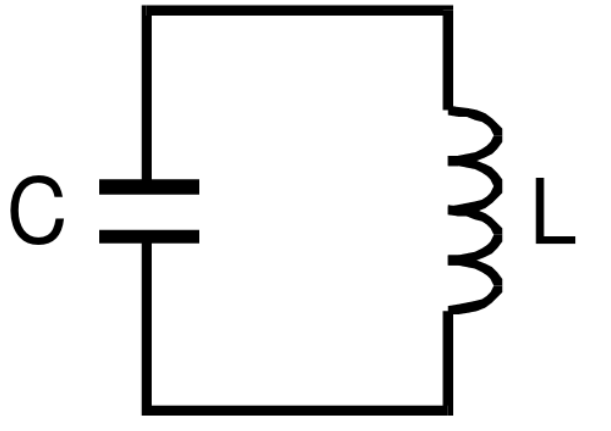
\includegraphics[width=\linewidth-300pt,height=\textheight-300pt,keepaspectratio]{content/images/CL.png}
\caption{Schaltskizze eines $LC$-Kreises \cite{V354}.}
\label{fig:LC_Kreis}
\end{figure}
   
\subsection{Der $RLC$-Kreis}

Der $RLC$-Kreis ist ein gedämpfter Schwingkreis und eine Erweiterung des $LC$-Kreises, in dem zusätzlich über einen ohmschen Widerstand $R$ Energie in Wärme umgesetzt wird. Die Kondensatorspannung $U_.C$ und die Stromstärke $I$ sind hier monoton fallende Funktionen der Zeit $t$. Das Schaltbild ist in Abbildung \ref{fig:RLC_Kreis} dargestellt.

\begin{figure}
\centering
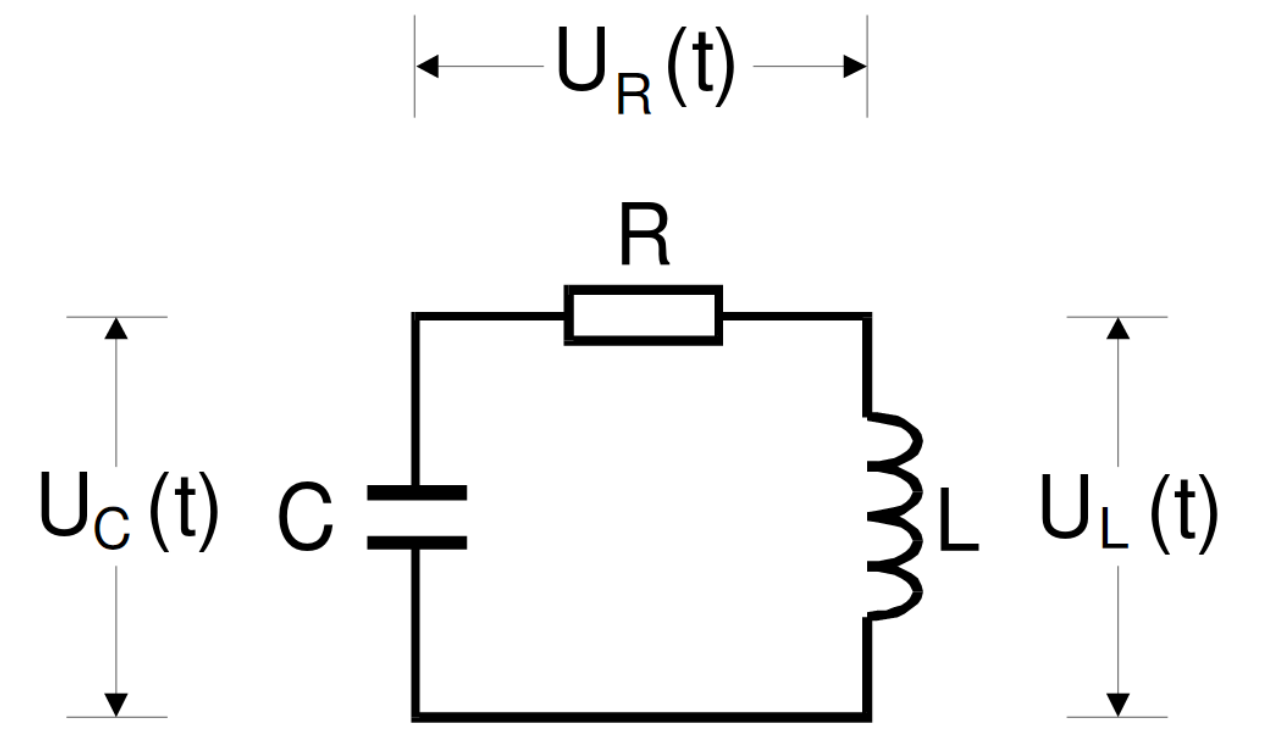
\includegraphics[width=\linewidth-200pt,height=\textheight-200pt,keepaspectratio]{content/images/RCL.png}
\caption{Schaltskizze eines $RCL$-Kreises \cite{V354}.}
\label{fig:RLC_Kreis}
\end{figure}
 
\noindent Mit den Kirchhoffschen Gesetzen folgt für $I$ eine lineare homogene Differentialgleichung zweiter Ordnung der Form:
\begin{equation}
\ddot{I} + \frac{R}{L} \dot{I} + \frac{1}{LC}I = 0\text{.} \label{eq:Diff_I}
\end{equation}
%Mit dem Ansatz
%\begin{equation}
%I = A\exp(\lambda t) \label{eq:I_Ans}
%\end{equation}
%lässt sich Gleichung \eqref{eq:Diff_I} lösen und für $\lambda$ ergibt sich:
%\begin{equation}
%\lambda_{1,2} = -\frac{R}{2L}\pm \sqrt{\frac{R^2}{4L^2}-\frac{1}{LC}}\text{.} \label{eq:lambda}
%\end{equation}
Mit der Dämpfungskonstanten
\begin{equation}
\gamma=\frac{R}{2L},\label{eq:gamma}
\end{equation}
der Kreisfrequenz des ungedämpften Systems
\[
\omega_.0 = \sqrt{\frac{1}{LC}}
\]
und der Kreisfrequenz des gedämpften Systems
\begin{equation}
\omega_.g=\sqrt{\gamma^2-\omega_.0^2}\label{eq:omega}
\end{equation}
ergibt sich die allgemeine Lösung von Gleichung \eqref{eq:Diff_I} zu:
\begin{equation}
I(t) = \exp(-\gamma t)\left(A_.1\exp(\omega_.g t)+A_.2\exp(-\omega_.g t)\right)\text{.} \label{eq:I}
\end{equation}
Die Konstanten $A_.1$ und $A_.2$ sind dabei von den Anfangsbedingungen abhängig.
In Gleichung \eqref{eq:I} ist zu erkennen, das sich für unterschiedliche $\omega_.g$ verschiedene Arten von Lösungen ergeben.\newline
Ist $\omega_.0>\gamma$, so wird $\omega_.g$ nach Gleichung \eqref{eq:omega} imaginär und die Lösung ist eine gedämpfte Schwingung der Form:
\begin{equation}
I(t) = A \exp(-\gamma t) \mathrm{cos}(\omega_.g t + \phi)\text{.} \label{eq:I2}
\end{equation}
Die Periodendauer $T$ und die Abklingdauer $\tau$ des schwingenden Systems ergeben sich zu:
\begin{equation}
T = \frac{2\pi}{\omega_.g} \text{\hspace{2em} und \hspace{2em}} \tau = \frac{2L}{R}\text{.}\label{eq:tau}
\end{equation}
Ist $\omega_.0<\gamma$, so ist $\omega_.g$ nach Gleichung \eqref{eq:omega} reel und es liegt eine Dämpfung vor, die nach hinreichender Zeit ein einfaches Relaxationsverhalten zeigt. Je nach Wahl von $A_.1$ und $A_.2$ kann die Funktion zuvor einen Extremalwert durchlaufen. Einige Beispiele sind in Abbildung \ref{fig:Daempfungen} dargestellt.

\begin{figure}
\centering
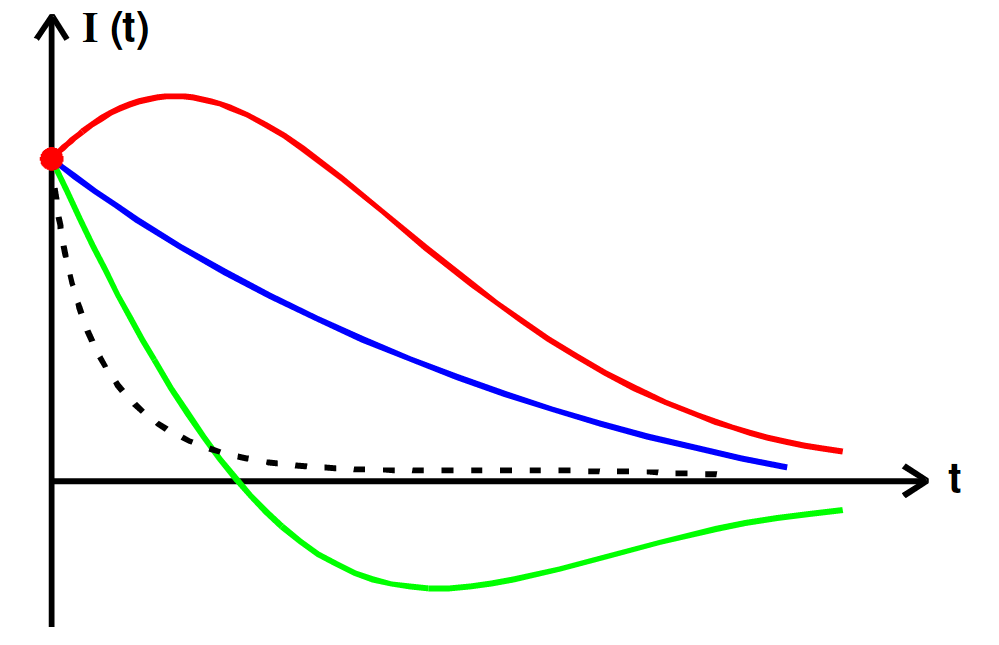
\includegraphics[width=\linewidth-200pt,height=\textheight-200pt,keepaspectratio]{content/images/daempfungen.png}
\caption{Relaxationsverhalten bei verschiedenen aperiodischen Dämpfungen \cite{V354}.}
\label{fig:Daempfungen}
\end{figure}

\noindent Ist $\omega_.0=\gamma$, so liegt der aperiodische Grenzfall vor. Hier fällt die Funktion, in Abbildung \ref{fig:Daempfungen} schwarz gestrichelt, am schnellsten ab und durchläuft kein Extremum.  

\subsection{Der periodisch angeregte $RLC$-Kreis}
\label{subsec:RLCPeriodischAngeregt}

Liegt an dem $RLC$-Kreis eine Wechselspannung $U$ der Form 
\[
U(t)=U_.0\mathrm{cos}(\omega t)
\]
mit der Kreisfrequenz $\omega$ und der Amplitude $U_.0$ an, so ergibt sich eine lineare inhomogene Differentialgleichung der Form:
\begin{equation}
LC\ddot{U}_.C + RC\dot{U}_.C + U_.C = U_.0\mathrm{cos}(\omega t)\text{.}\label{eq:U_Diff}
\end{equation}
Es ergibt sich mit der Lösung von Gleichung \eqref{eq:U_Diff} für für die Amplitude $A_.C$ der Kondensatorspannung eine Abhängigkeit zu $\omega$ von:
\begin{equation}
A_C(\omega) = \frac{U_.0}{\sqrt{(1-LC\omega^2)^2 + \omega^2R^2C^2}}\text{.}\label{AC}
\end{equation}
Es zeigt sich zudem eine Phasenverschiebung $\phi$ zwischen $U_C$ und $U$. Für diese gilt:
\begin{align}
\phi(\omega) 	&= \arctan\left( \frac{-\omega RC}{1-LC \omega^2}\right)\\
				&= \omega \Delta t\text{.}\label{phi}
\end{align}
Dabei ist $\Delta t$ der Abstand der Extremstellen der beiden Spannungskurven, wenn diese in einem Graphen dargestellt werden.\newline
Nach Gleichung \eqref{AC} geht $A_.C$ für $\omega \to \infty$ gegen $0$ und für $\omega \to 0$ gegen $U_.0$.
Für die Resonanzfrequenz $\omega_.{res}$ erreicht $U_.C$ einen Maximalwert, welcher größer als $U_.0$ sein kann. Für $\omega_.{res}$ gilt:
\begin{equation}
\omega_.{res} = \sqrt{\frac{1}{LC}-\frac{R^2}{2L^2}}\text{.}
\end{equation}
Ist die Dämpfung gering, dann gilt
\[
\frac{R^2}{2L^2}<<\frac{1}{LC}
\]
und $A_.{C,max}$ berechnet sich nach:
\begin{equation}
A_.{C,max} = qU_.0\text{.}
\end{equation}
Dabei bezeichnet man 
\begin{equation}
q = \frac{1}{\omega_.0RC}
\end{equation}
als die Güte des Systems. Ist $R$ verschwindend gering, so strebt $A_.{C,max}$ gegen unendlich und es kommt zur Resonanzkatastrophe.\newline
Die Breite $B$ der Resonanzkurve wird durch die Differenz der Frequenzen beschrieben, bei denen $A_.C$ den Wert $\frac{A_.{C,max}}{\sqrt{2}}$ erreicht. Diese Fallen mit den Frequenzen zusammen, bei denen die Phasendifferenz $\phi=\frac{pi}{2}\pm\frac{pi}{4}$ ist. Sie berechnen sich nach:
\begin{equation*}
\omega_.{1,2} = \pm \frac{R}{2L} + \sqrt{\frac{R^2}{4L^2} + \frac{1}{LC}}\text{.}
\end{equation*}
Für die Breite $B$ folgt:
\begin{equation}
B = \omega_.1-\omega_.2 = \frac{R}{L}\text{.}
\end{equation}
Für eine starke Dämpfung existiert keine Resonanzfrequenz. Ist $\omega$ ausreichend groß, so ist eine $\frac{1}{\omega^2}$ Abhängigkeit von $A_.C$ zu erkennen, weshalb der $RLC$-Kreis in diesem Fall als Tiefpassfilter verwendet werden kann. 